

\begin{figure}
    \centering
        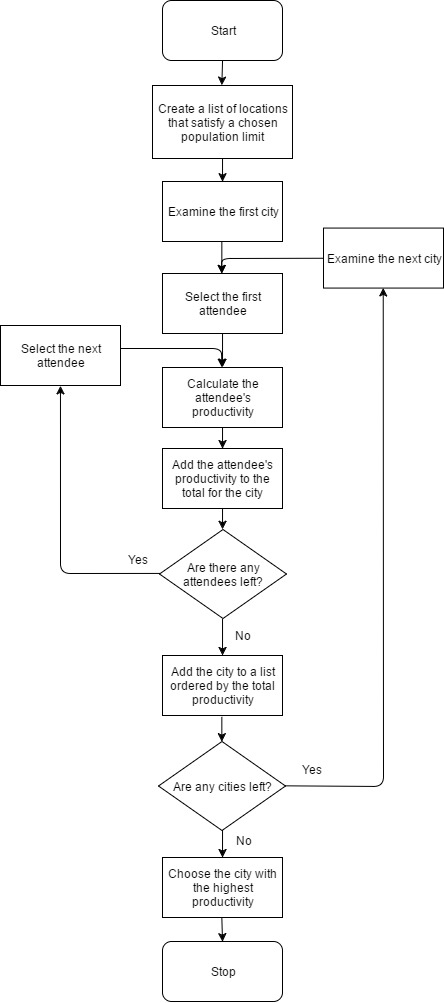
\includegraphics[width=\textwidth,height=0.95\textheight,keepaspectratio]{diagram}
    \caption{The flowchart representation of our discrete algorithm}
\end{figure}

The zoning algorithm turned out to be too imprecise and the only way to overcome it's limitations and achieve higher precision is to consider all factors for every area examined. Furthermore, we wanted to prevent a situation, where an ideal location would be lost in an unfavorable area, if possible. This led us to the need of examining every potentially suitable place by itself and not as a part of a larger area.

At first glance this may seem impossible, since there is an astronomical amount of places on Earth. Thankfully, we can limit our search somewhat, since a meeting cannot take place just anywhere. A certain level of base infrastructure is necessary to achieve the best working conditions and productivity. As a result, we will limit ourselves to only examining areas with urban development. Furthermore, we will filter out all municipalities without sufficient population. This value can be adjusted for the needs of the exact meeting, but for now the threshold is going to be set at around $50$ thousand inhabitants. This limit should ensure good accessibility, accommodation and services. Now we are left with roughly over $7000$ cities around the world to choose from.

We can calculate the productivity of every attendant of the meeting in every examined city using our models for each considered factor separately for each of the three days. Next, we will sum up the productivities for every city and compare them. The result of this algorithm will be a list of cities above our threshold ordered by their respective productivities.

In other words, our algorithm will iterate through all cities, then through all days of the meeting, then through attendees, and finally individual factors. This process may seem very resource intensive, however,
thanks to the filtering of possible places we implemented, the computation is almost instantaneous.

